
%-------------------------------------------------------------
%			PAGE BUILDER
%-------------------------------------------------------------

\mcchap{Integrazione Page Builder}{cap:pb}

Per passare ad una gestione più semplice delle pagine da parte dei content,
 è stato chiesto di cercare qualche sistema che permettesse una suddivisione
della pagina in componenti facilmente editabili e riutilizzabili.

Le esigenze principali erano:
\begin{itemize}
\item modificare il contenuto delle componenti da interfaccia grafica e non 
editando il codice HTML.
\item poter creare semplicemente copie delle componenti già create
\item poter spostare le varie componenti con \emph{drag and drop} e avere
feedback visivo immediato della modifica della pagina
\end{itemize}

Per questo mi è stato consigliato di fare una ricerca tra le varie soluzioni disponibli
nella ampia libreria di plugin di Wordpress.


Dopo aver analizzato i vari plugin disponibili, è stata individuata una soluzione open source chiamata \emph{Page Builder by
Site Origin}\cite{PB} che soddisfava le esigenze.

\section{Page Builder by Site Origin}

Il plugin \emph{Page Builder} permette la suddivisione della pagina in colonne all'interno delle quali
si possono inserire delle componenti.

Queste componenti possono essere duplicate, modificate aprendo il form della componente e spostate
con drag and drop.


\begin{figure}
  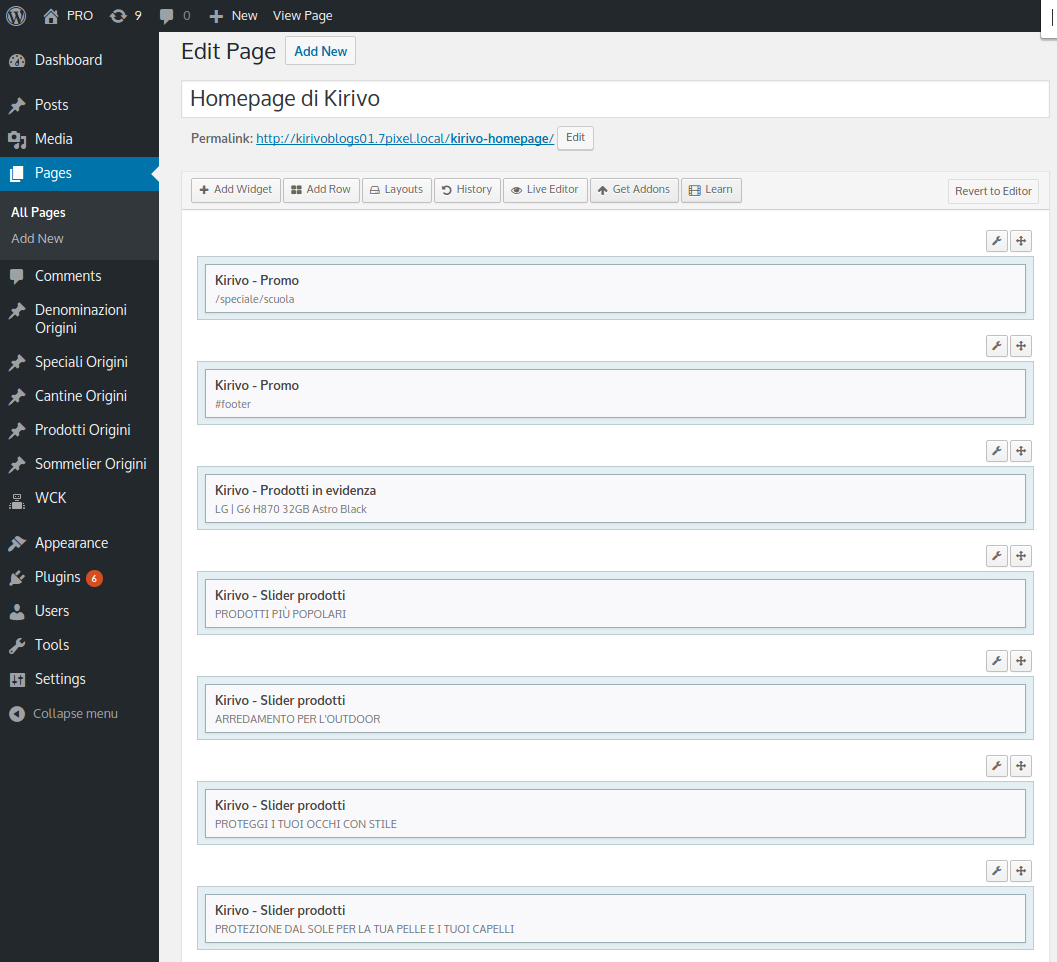
\includegraphics[width=\textwidth]{figure/pagebuilder.png}
  \caption{L'interfaccia di editing di \emph{Page Builder} per la homepage di Kirivo permette
  la suddivisione della pagina in componenti e la loro copia e modifica.}
  \label{fig:wsource}
\end{figure}


Il vantaggio di questo plugin rispetto ad altri che permettono la suddivisione della pagine è che all'interno delle colonne,
oltre a poter inserire delle componenti standard fornite dal plugin, si possono anche inserire i Widget di Wordpress.

\section{Widget}
I \emph{Widget} sono delle componenti riutilizzabili che possono essere aggiunte a qualsiasi
tipo di pagina Wordpress. 

Wordpress contiene già al suo interno numerosi Widget già pronti all'uso, classici esempi di Widget sono le icone per i link ai social network o un'anteprima di un post creato, tuttavia è possibile creare Widget
personalizzati.

Per creare un Widget bisogna implementare una sottoclasse di WP\_Widget\cite{WPWID}
e sovrascrivere il metodo \emph{Widget} dove verrà restituito il contenuto HTML che la pagina deve restituire quando quel Widget viene incluso in una pagina
e, se si vuole del contenuto dinamico, bisogna sovrascrivere \emph{form} dove viene creato il form HTML che verrà visualizzato dai content per modificare le
parti dinamiche delle componenti.

Le componenti compilate nel form vengono poi utilizzate dal metodo \emph{Widget}.


\lstinputlisting[style=customphp, basicstyle=\tiny, language=Php]{code/exampleWidget.php}
\emph{Una semplice implementazione di un Widget che stampa un titolo dinamicamente}


\begin{figure}
  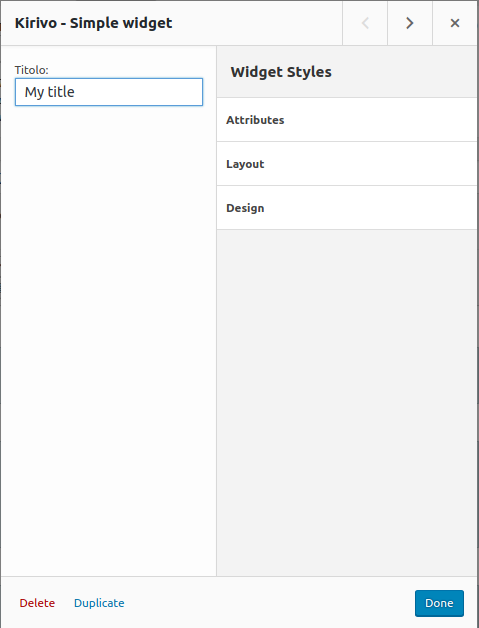
\includegraphics[width=0.6\textwidth]{figure/wid_form.png}
  \caption{Il form che viene visualizzato per modificare i dati del Widget.}
  \label{fig:wform}
\end{figure}
\begin{figure}
  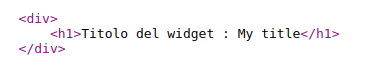
\includegraphics[width=0.7\textwidth]{figure/sourcewid.png}
  \caption{Porzione di sorgente di una pagina che utilizza il Widget compilato come in \ref{fig:wform}.}
  \label{fig:wsource}
\end{figure}

\newpage

\section{Inizializzazione}
Per inizializzare i Widget bisogna aggiungere una action\cite{WPACTION}, ovvero un meccanismo offerto da Wordpress per aggiungere dei comportamenti
prestabiliti,  chiamata \emph{init\_Widget} che permette di registrare i Widget creati.

La sintassi per aggiungere un action in Wordpress è la seguente
\begin{verbatim}
add_action('nome_action','nome_della_funzione_implementata')
\end{verbatim}

Per far in modo di non dover aggiungere manualmente un Widget al file di inizializzazione ogni volta che se ne crea uno nuovo, è
stato implementato un script di inizializzazione che va all'interno delle cartelle \emph{widget\_orgini} e \emph{widget\_kirivo} e aggiunge e registra tutti
i Widget che trova all'interno di queste cartelle, per individuare un Widget all'interno della cartella viene fatto pattern-matching per i file che terminano con \emph{Widget.php}.

\lstinputlisting[style=customphp, basicstyle=\tiny, language=Php]{code/intializeWidget.php}
\emph{Il file initialize\_Widget.php che permette la registrazione di tutti i Widgets}

\section{Implementazione Widget}
Per implementare i Widget necessari per le homepage sono state isolate le componenti HTML necessarie e per ognuna
di queste è stato creato un Widget poi, per ognuna di queste è stato creato il suo form per editare le componenti necessarie.

Ci sono due categorie principali di Widget
\begin{itemize}
\item Widget che non contengono prodotti.
\item Widget che contengono prodotti.
\end{itemize}

Per implementare i Widget che non contengono prodotti, come ad esempio il Widget \emph{Origni - Speciale}, è stato messo all'interno del metodo \emph{Widget} direttamente
l'HTML di quella componente con eventuale contenuto dinamico stampato in php e nel metodo \emph{form} aggiunto l'HTML per gli input necessari.

\begin{figure}
  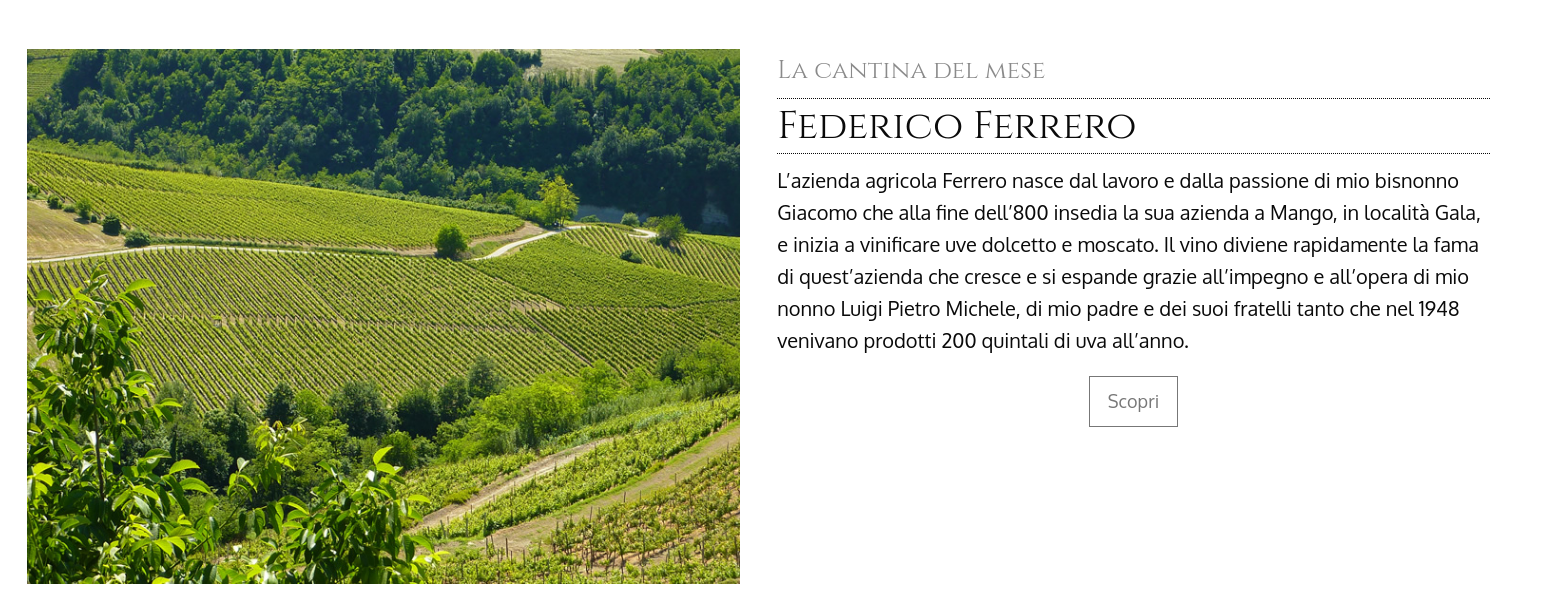
\includegraphics[width=\textwidth]{figure/ospec.png}
  \caption{Contenuto renderizzato dal Widget \emph{Origni - Speciale}.}
  \label{fig:ospec1}
\end{figure}

\begin{lstlisting}[style=customphp, basicstyle=\tiny, language=Php,caption={Codice del Widget \emph{Origini - Speciale}}] 
<?php
class specialWidget extends WP_Widget {
  function __construct() {
    parent::__construct( false, 'Origini - Speciale');
  }


  function Widget( $args, $instance ) {;
    $image = ! empty( $instance['img-link'] ) ? $instance['img-link'] : '';
    ?>
    <section id="hp_editorial_contents" class="bg_white">
    <div class="row paragraph_vertically_spaced">
      <div class="small-12 medium-6 columns">
        <div class="hp_box">
          <a href="<?php echo $instance['link']?>">
            <picture class="tile_article_image">
              <img src="<?php echo $image?>" alt="descrizione dell&#39;immagine">
            </picture>
          </a>
        </div>
      </div>
      <div class="small-12 medium-6 columns">
        <div class="hp_box">
          <div class="hp_article_box">
            <h5 class="subheader"><?php echo $instance['subtitle']?></h5>
            <h3 class="dotted_bordered"><?php echo $instance['title']?></h3>
            <h4 class="subheader"></h4>
            <p class="hp_article"><?php echo $instance['description']?></p>
          </div>
          <div class="row hp_box_more text-center">
            <a href="<?php echo $instance['link']?>" class="hollow ">Scopri</a>
          </div>
        </div>
      </div>
    </div>
    </section><?php
  }


  function form( $instance ) {
    $title = esc_attr($instance['title']);
    $image = ! empty( $instance['img-link'] ) ? $instance['img-link'] : '';?>
    <p><label for="<?php echo $this->get_field_id('subtitle');?>"></label>
        Sottotitolo: </p><input id="<?php echo $this->get_field_id('subtitle');?>" 
        	name="<?php echo $this->get_field_name('subtitle');?>" type="text" 
        	value="<?php echo $instance['subtitle']; ?>" />
    </p>
    <p><label for="<?php echo $this->get_field_id('title');?>"></label>
        Titolo:</p> <input class="required" id="<?php echo $this->get_field_id('title');?>"
        	name="<?php echo $this->get_field_name('title');?>" type="text" 
        	value="<?php echo $title; ?>" />
    </label>
    <p><label for="<?php echo $this->get_field_id('description');?>"></label>
        Descrizione:</p> <input id="<?php echo $this->get_field_id('description');?>" 
        	name="<?php echo $this->get_field_name('description');?>" type="text" 
        	value="<?php echo $instance['description']; ?>" />
    </p>
    <p><label for="<?php echo $this->get_field_id('link');?>"></label>
        Link:</p> <input class="required" id="<?php echo $this->get_field_id('link');?>" 
        name="<?php echo $this->get_field_name('link');?>" type="text" 
        value="<?php echo $instance['link']; ?>" />
    </p>
    <p>
      <label for="<?php echo $this->get_field_id( 'img-link' ); ?>"></label>
      <input id="<?php echo $this->get_field_id( 'img-link' ); ?>" 
	      name="<?php echo $this->get_field_name( 'img-link' ); ?>" type="text" 
	      value="<?php echo esc_url( $image ); ?>" />
      <button class="upload_image_button button button-primary">
      	Upload or select image
      </button>
    </p>
    <?php
  }
}
\end{lstlisting}

Per i \emph{Widget} che contengono prodotti invece, all'interno del metodo \emph{Widget} non è stato inserito il codice HTML con il template
di ogni prodotto ma è stato messo il tag \emph{dynamic} i cui attributi sono popolati dinamicamente in base a come viene compilato il form della componente.
Una volta che il server Kiruby prende una pagina Wordpress e trova il dynamic tag allora provvede a sostituire il tag con le schede con le informazioni
di tutti i prodotti specificati.
\newpage

\begin{lstlisting}[style=customphp, basicstyle=\tiny, language=Php,caption={Il metodo \emph{Widget} di \emph{Origini - Slider prodotti} stampa il dynamic tag che verrà letto da Kiruby e sostituito con l'HTML dei prodotti}] 
function Widget( $args, $instance ) {?>
  <dynamic type="OriginiHomeSpecialProductsBox" product_ids="<?php echo $instance['ids']?>" 
    title="<?php echo $instance['title']?>" subtitle="<?php echo $instance['subtitle']?>" 
    link="<?php echo $instance['scopri-link']?>" no_slack='true' />
  <?php}
\end{lstlisting}\